\section{Theoretical Foundations}
\label{sec:theory}
%As discussed in Section~\ref{sec:implementation}, there are two different types of analysis that can be performed on a fault model. The initial stages of the project implemented a \textit{Verify in the Presence of Faults} analysis that returned a single counterexample if a fault caused violation of a property. In later stages of this project, this was extended in order to collect all such fault combinations that caused these violations, \textit{Generate Minimal Cut Sets}. 

There are two different types of fault analysis that can be performed on a fault model, \textit{Verification in the Presence of Faults}, and \textit{Generate Minimal Cut Sets}, as introduced in Section~\ref{sec:implementation}. The theoretical foundations used to verify a model in the presence of faults relies on AGREE and the theory underlying the assume guarantee environment~\cite{cofer2012compositional}; this theory will not be discussed further in this report. The underlying theoretical framework used in the generation of minimal cut sets is described in detail in this section. 



%\subsection{Theory of Verification in the presence of Faults}
\label{sec:verify_theory}
The theoretical foundations used to verify a model in the presence of faults relies on AGREE and the theory used to prove the assume guarantee environment~\cite{cofer2012compositional}. 

\begin{comment}

Assuming that dependent faults have been collected and mapped appropriately, they are in the following form: \\
$\{\{f_1 \rightarrow\{f_3, f_7\}, f_5 \rightarrow\{f_2\},...\}$ meaning that $f_3$ and $f_7$ are dependent on $f_1$ and so on.

We make the assumption that there are no nested dependencies. To clarify this, we cannot have something of the form: \\
$f_1 \rightarrow \{f_3, f_5\}$\\
$f_3 \rightarrow \{f_4\}$

If this is the case, the user must define the dependency as follows: \\
$f_1 \rightarrow \{f_3, f_4, f_5\}$. 

\begin{algorithm}[H]
	% \KwData{this text}
	% \KwResult{how to write algorithm with \LaTeX2e }
	Input: $F$: map between allowable combination $F_i$ and associated probability (initially zero) \;
	Output: $F$: map between allowable combinations with dependencies and associated probability (nonzero) \;
	$newMCS =$ empty list \;
	$p=1$ \;
	\For{all allowable fault combinations $F_i \in F$}{
		Remove $F_i$ from $F$ \;
		\For{all $f_i \in MCS$ }{
		    \If{$f$ is key in dependency map}{
		    	$p = p*prob(f)$ \;
		    	append $f$ to $newMCS$ \;
		    	append dependent faults triggered by $f$ to $newMCS$ \;
		    	\For{all depFaults triggered by $f$ activation}{
		    		\If{depFault $\in MCS$}{
		    			remove depFault from $MCS$ \;
		    		}%end if depFault is in MCS
		    	} %end for all dep faults triggered
		    } %end if f is a key in the dependency map
		} % end for all faults in MCS
		Append $F_i \rightarrow p$ to $F$ \;
	}%end for all combos in F
	return $newMCS$ as the completed MCS \;
	\caption{Incorporate Dependencies}
	\label{alg:dep_alg}
\end{algorithm}

\end{comment}
%\subsection{Theory Behind the Generation of Minimal Cut Sets}
\label{sec:generate_theory}
The following sections describe in detail the background information, definitions, theory, and algorithms used in the process of generating minimal cut sets through the use of the All-MIVC algorithm.

\subsection{Fault Tree Analysis} 
The use of fault trees are common in many safety assessment processes and the ability to generate the cut sets needed for the construction of the fault tree is a useful part of any safety analysis tool. The fault tree is a safety artifact commonly referenced in requirement protocol documents such as ARP4761, ARP4754, and AIR6110~\cite{SAE:ARP4761,SAE:ARP4754A,AIR6110}.

% There are two main types of fault tree analysis that we differentiate here as \textit{qualitative} analysis and \textit{quantitative} analysis. In qualitative analysis, the structure of the fault tree is considered and the cut sets are a way to indicate which combinations of component failures will cause the system to fail. On the other hand, in quantitative analysis the probability of the TLE is calculated given the probability of occurance of the basic events. By being able to generate cut sets based on both probability and cardinality, this allows for either form of FTA to be created. 

A Fault Tree (FT) is a directed acyclic graph whose leaves model component failures and whose gates model failure propagation~\cite{0f356f05e72f43018211b36f97c8854a}. The system failure under examination is the root of the tree and is called the Top Level Event (TLE). The node types in a fault tree are \textit{events} and \textit{gates}. An event is an occurrence within the system, typically the failure of a subsystem down to an individual component. Events can be grouped into Basic Events (BEs), which occur independently, and \textit{intermediate events} which occur dependently and are caused by one or more other events~\cite{historyFTA}.  These events model the failure of the system (or subsystem) under consideration. The gates represent how failures propagate through the system and how failures in subsystems can cause system wide failures. The two main logic symbols used are the Boolean logic AND-gates and OR-gates. An AND-gate is used when the undesired top level event can only occur when all the lower conditions are true. The OR-gate is used when the undesired event can occur if any one or more of the next lower conditions is true. This is not a comprehensive list of gate types, but we focus our attention on these two common gate types. 
\begin{figure}[h]
\begin{center}
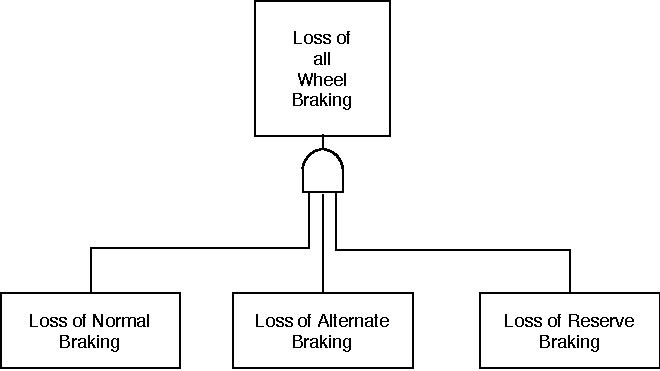
\includegraphics[width=8cm]{images/introFT2.pdf}
\caption{A simple fault tree} \label{fig:introFT}
\end{center}
\end{figure}

Figure~\ref{fig:introFT} shows a simple example of a fault tree based on SAE ARP4761~\cite{SAE:ARP4761}. In this example, the top level event corresponds to an aircraft losing all wheel braking. In order for this event to occur, all of the basic events must occur. This is seen through the use of the AND gate below the top level event. The gates in the fault tree describe how failures propagate through the system. Each gate has one output and one or more inputs. In Figure~\ref{fig:introFT}, the AND gate has three inputs and one output. The leaves of the tree represent the basic events of the system. %and 
In the case of this fault tree, these three events are also the Minimal Cut Sets (MinCutSets) for this top level event. A MinCutSet is the minimal set of basic events that must occur together in order to cause the TLE to occur. Generating and analyzing these MinCutSets is important to FTA and has been an active area of interest in the research community since fault trees were first described in Bell Labs in 1961~\cite{historyFTA,0f356f05e72f43018211b36f97c8854a}. 

There are two main types of fault tree analysis that we differentiate here as \textit{qualitative} analysis and \textit{quantitative} analysis. In qualitative analysis, the structure of the fault tree is considered and the MinCutSets are a way to indicate which combinations of component failures will cause the system to fail. On the other hand, in quantitative analysis the probability of the TLE is calculated given the probability of occurrence of the basic events. By being able to generate MinCutSets
based on both cardinality and probability, this allows for either form of FTA to be created. 


%\subsection{Inductive Validity Cores}

%Given a complex model, it is often useful to extract traceability information related to the proof, in other words, which portions of the model were necessary to construct the proof. An algorithm was introduced by Ghassabani, et. al. to provide Inductive Validity Cores (IVCs) as a way to determine which model elements are necessary for the inductive proofs of the safety properties for sequential systems~\cite{GhassabaniGW16}. Given a safety property of the system, a model checker can be invoked in order to construct a proof of the property. The IVC generation algorithm extracts traceability information from the proof process and returns a minimal set of the model elements required in order to prove the property. Later research extended this algorithm in order to produce all IVC elements~\cite{Ghassabani2017EfficientGO}. 

%The IVC algorithm considers a constraint system consisting of the assumptions and contracts of system components and the negation of the safety property of interest (i.e. the top level event). It then collects what are called Minimal Unsatisfiable Subsets (MUSs) of this constraint system; these are the minimal explanations of the constraint systems infeasibility in terms of the \textit{negation} of the safety property. Equivalently, these are the minimal model elements necessary to proof the safety property.

%In section \ref{sec:definitions}, we show the formal definitions of IVCs in detail. \\

%Our approach utilizes a few tools in order to generate the artifacts of interest and a brief background will be helpful. and hence the rest of the background section consists of a brief description of AADL, AGREE, and the SOTERIA tools and languages. 

%\subsection{Architecture Analysis and Design Language}
%We are using the Architectural Analysis and Design Language (AADL) to construct system architecture models.  AADL is an SAE International standard that defines a language and provides a unifying framework for describing the system architecture for ``performance-critical, embedded, real-time systems''~\cite{AADL_Standard,FeilerModelBasedEngineering2012}. From its conception, AADL has been designed for the design and construction of avionics systems.  Rather than being merely descriptive, AADL models can be made specific enough to support system-level code generation.  Thus, results from analyses conducted, including the new safety analysis proposed here, correspond to the system that will be built from the model.  

%An AADL model describes a system in terms of a hierarchy of components and their interconnections, where each component can either represent a logical entity (e.g., application software functions, data) or a physical entity (e.g., buses, processors). An AADL model can be extended with language annexes to provide a richer set of modeling elements for various system design and analysis needs (e.g., performance-related characteristics, configuration settings, dynamic behaviors). The language definition is sufficiently rigorous to support formal analysis tools that allow for early phase error/fault detection.

%\subsection{Compositional Analysis} Compositional analysis of systems was introduced in order to address the scalability of model checking large software systems. Monolithic verification and compositional verification are two ways that mathematical verification of component properties can be performed. In monolithic analysis, the model is flattened and the top level properties are proved using only the leaf level contracts of the components. On the other hand, the analysis can be performed compositionally following the architecture hierarchy such that analysis at a higher level is based on the components at the next lower level. The idea is to partition the formal analysis of a system architecture into verification tasks that correspond into the decomposition of the architecture. A component contract is an assume-guarantee pair. Intuitively, the meaning of a pair is: if the assumption is true, then the component will ensure that the guarantee is true. The components of a system are organized hierarchically and each layer of the architecture is viewed a system. For any given layer, the proof consists of demonstrating that the system guarantee is provable given the guarantees of its direct subcomponents and the system assumptions. This proof is performed one layer at a time starting from the top level of the system. When compared to monolithic analysis (i.e., analysis of the flattened model composed of all components), the compositional approach allows the analysis to scale to much larger systems~\cite{NFM2012:CoGaMiWhLaLu}. 

%\subsection{Assume Guarantee Reasoning Environment}
%The Assume Guarantee Reasoning Environment (AGREE) is a tool for formal analysis of behaviors in AADL models~\cite{NFM2012:CoGaMiWhLaLu}.  It is implemented as an AADL annex and annotates AADL components with formal behavioral contracts. Each component's contracts can include assumptions and guarantees about the component's inputs and outputs respectively, as well as predicates describing how the state of the component evolves over time.

%AGREE translates an AADL model and the behavioral contracts into Lustre~\cite{Halbwachs91:IEEE} and then queries a user-selected model checker to conduct the back-end analysis. The analysis can be performed compositionally or monolithically.

%\subsection{Safety Annex for AADL}
%The Safety Annex for AADL is a tool that provides the ability to reason about faults and faulty component behaviors in AADL models~\cite{Stewart17:IMBSA,SATechReport}. In the Safety Annex approach, formal assume-guarantee contracts are used to define the nominal behavior of system components. The nominal model is verified using AGREE. The Safety Annex weaves faults into the nominal model and analyzes the behavior of the system in the presence of faults. The tool supports behavioral specification of faults and their implicit propagation through behavioral relationships in the model as well as provides support to capture binding relationships between hardware and software compönents of the system. 

\begin{comment}
\subsection{SOTERIA}
The Safe and Optimal Techniques Enabling Recovery, Integrity, and Assurance (SOTERIA) tool is used to perform safety analysis of Integrated Modular Avionics (IMA) systems~\cite{SOTERIAproject}. In the SOTERIA project, a compositional modeling language was developed and this language is used as input in order to automatically synthesize the qualitative and quantitative safety analyses. The tool is compositional in that it requires safety aspects at each component level which enables the generation of compositional fault trees. 

\begin{figure}[h]
\begin{center}
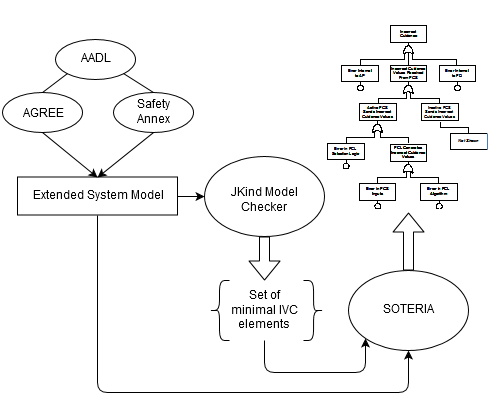
\includegraphics[width=8cm]{images/processFTA.png}
\caption{Outline of the fault tree generation process} \label{fig:processFTA}
\end{center}
\end{figure}

\end{comment}





\subsection{Definitions}
\label{sec:definitions}
Intuitively a constraint system contains the contracts that constrain component behavior and faults that are defined over these components. In the case of a nominal model augmented with faults, a constraint system is defined as follows. Let $F$ be the set of all fault activation literals defined in the model and $G$ be the set of all component contracts (guarantees). 

\begin{definition}A constraint system $C = \{C_1,C_2,...,C_n\}$ where for $i \in \{1,...,n\}$, $C_i$ has the following constraints for any $f_j \in F$ and $g_k \in G$ with regard to the top level property $P$: 
\begin{center}
$C_i \in \left\{ \begin{array}{ll}
	f_j :&  inactive\\
	g_k :& true\\
	P :& false\\
\end{array}\right.$	
\end{center}
\label{def:constraintsystem}
\end{definition}

Given a state space $S$, a transition system $(I,T)$ consists of the initial state predicate $I : S \rightarrow \{0,1\}$ and a transition step predicate $T : S \times S \rightarrow \{0,1\}$. Reachability for $(I,T)$ is defined as the smallest predicate $R : S \rightarrow \{0,1\}$ that satisfies the following formulas:
\begin{center}
$\forall s. I(s) \Rightarrow R(s)$\\
$\forall s, s' .  R \land T(s,s') \Rightarrow R(s')$\\
\end{center}
A safety property $\mathcal{P} : S \to \{0,1\}$ is a state predicate. A safety property $\mathcal{P}$ holds on a transition system $(I,T)$ if it holds on all reachable states. More formally, $\forall s . R(s) \Rightarrow \mathcal{P}(s)$. When this is the case, we write $(I,T) \vdash\mathcal{P}$~\cite{Ghassabani2017EfficientGO}. 

Given a transition system that satisfies a safety property $P$, it is possible to find which model elements are necessary for satisfying the safety property through the use of the \textit{All Minimal Inductive Validity Cores All-MIVCs} algorithms~\cite{Ghassabani2017EfficientGO,bendik2018online}. This algorithm collects all minimal unsatisfiable subsets of a given transition system in terms of the negation of the top level property. The minimal unsatisfiable subsets consist of component contracts constrained to \textit{true}. When the constraints on these model elements are removed from the constraint system $C$, this results in an UNSAT system. This can be seen as the minimal explanation of the constraint systems infeasibility. Recall that this constraint system is in terms of the \textit{negation} of the safety property. Thus, this algorithm provides all model elements required for the proof of the safety property. 

We utilize this algorithm by providing not only component contracts (constrained to \textit{true}) as model elements, but also fault activation literals constrained to \textit{false}. Thus the resulting MIVCs will contain the required contracts and constrained fault activation literals in order to prove the safety property. This information is used throughout this section to provide the underlying theory behind the generation of minimal cut sets from all MIVCs. 

Definitions 1-3 are taken from research by Liffiton et. al.~\cite{liffiton2016fast}. 

\begin{definition} : A Minimal Unsatisfiable Subset ($MUS$) of a constraint system $C$ is :\\
 $\{MUS \subseteq C$ $|$ $MUS$ is UNSAT and $\forall c \in MUS$: $MUS \setminus \{c\}$ is SAT$\}$. This is the minimal explaination of the constraint systems infeasability. 
\end{definition}

A closely related set is a \textit{minimal correction set} (MCS). The MCSs describe the minimal set of model elements for which if constraints are removed, the constraint system is satisfied. For constraint system $C$, this corresponds to which faults are not constrained to inactive (and are hence active) and violated contracts which lead to the violation of the safety property. In other words, the minimal set of active faults and/or violated properties that lead to the top level event.  

\begin{definition} : A Minimal Correction Set ($MCS$) of a constraint system $C$ is :\\
 $\{MCS \subseteq C$ $|$ $C \setminus MCS$ is SAT and $\forall S \subset MCS$ : $C \setminus S$ is UNSAT$\}$. A MCS can be seen to ``correct'' the infeasability of the constraint system.
\end{definition}

A duality exists between MUSs of a constraint system and MCSs as established by Reiter \cite{reiter1987theory}. This duality is defined in terms of \textit{minimal hitting sets}. A hitting set of a collection of sets $A$ is a set $H$ such that every set in $A$ is ``hit'' be $H$; $H$ contains at least one element from every set in $A$ \cite{liffiton2016fast}. The MCSs can be generated from the MUSs if all MUSs are known. Thus, the use of the All-MIVCs algorithm is required. 

\begin{definition}: Given a collection of sets $K$, a hitting set for $K$ is a set $H \subseteq \cup_{S \in K} S$ such that $H \cap S \neq \emptyset$ for each $S  \in K$. A hitting set for $K$ is minimal if and only if no proper subset of it is a hitting set for $K$. 
\end{definition}

Utilizing this approach, the MCSs are generated from the MUSs that are provided by the All-MIVCs algorithm~\cite{Ghassabani2017EfficientGO} and a minimal hitting set algorithm developed by Murakami et. al.~\cite{murakami2013efficient,gainer2017minimal}. \\

A Minimal Cut Set ($MinCutSet$) is a minimal collection of faults that lead to the violation of the safety property (or in other words, lead to the top level event in the fault tree). We define a minimal cut set consistently with much of the research in this field~\cite{0f356f05e72f43018211b36f97c8854a,historyFTA}

\begin{definition} :  A Minimal Cut Set can be defined as the set of faults in a system that cause the violation of the safety property. Furthermore, any strict subset of these faults will not cause violation of the safety property. 
\end{definition}








\subsection{Transformation of All-MIVCs into Minimal Cut Sets}
\label{sec:transformation}
%The IVCs
All Minimal Inductive Validity Cores are collected by use of the All-MIVCs algorithm~\cite{Ghassabani2017EfficientGO}. These are all of the Minimal Unsatisfiable Subsets (MUSs) which can be used as input to the Minimal Hitting Set algorithm~\cite{murakami2013efficient,gainer2017minimal} in order to collect all Minimal Correction Sets (MCSs). The MCSs are then transformed into Minimal Cut Sets according to the following theoretical results. 

The definition of the constraint system follows Definition 1 in Section~\ref{sec:definitions}.

\begin{theorem}  The MinCutSet can be generated by the transformation of the Minimal Correction Set (MCS).

\begin{proof}  All $MCS$s are of the form $MCS = G \cup \overline{F}$ where $G$ consists of contracts in the system and $\overline{F}$ consists of faults constrained to false for constraint system $C$. 

\textbf{Case 1}: $G = \emptyset$\\
In the leaf level of the system, only constrained faults are contained in $MCS$. According to the defintion of an $MCS$, upon removing the constraints from $C$ of the elements contained in the $MCS$, the constraint system is satisfiable. Furthermore, the $MCS$ is the minimal such set. Thus, the constraint system with the \textit{active} faults from $MCS$ will cause the \textit{negation} of the safety property to be satisfied. The set of unconstrained faults found in the $MCS$ is the defintion of a minimal cut set. 

\textbf{Case 2}: $G \neq \emptyset$\\
Let $MCS = \{\lnot f_1,...,\lnot f_n,g_1,...,g_m\}$ where $f_j \in F$ and $g_k \in G$ and $\lnot f$ is a fault activation literal $f$ constrained to \textit{false}. 
For all $g_i \in MCS$, we know that the validity of $g_k$ is required in the proof of the top level property $P$ due to its generation through the All-MIVCs algorithm. For $g_1 \in MCS$, there exists a set containing all minimal cut sets of $g_1$. Call this $Cut(g_1) = \{F_{1i} \subseteq F | F_{1i}$ is a min cut set for $g_1, i = 1,...,p_1\}$. 

Replace $g_1$ with $F_{1i}$ for all $i = 1,...,p_1$. This produces $p_1$ new MCSs of the form:
\begin{center}
$\{f_1,...,f_n,F_{11},...,g_m\}$\\
$\{f_1,...,f_n,F_{12},...,g_m\}$\\
$\vdots$\\
$\{f_1,...,f_n,F_{1p_1},...,g_m\}$\\
\end{center}

Perform this replacement for all $g_k \in MCS$, $k=1,...,m$. %This produces at most $|p_1| \times \hdots \times |p_m|$ MCSs containing only faults. 

Let $I_\alpha$ be one of the sets generated by full replacement of all contracts in some $MCS_\alpha$ with their respective minimal cut set and all fault activation literals constrainted to \textit{true}.\\

\textit{Claim: $I_\alpha$ is a minimal cut set for safety property $P$}\\
By the definition of $MCS_\alpha$, $C\setminus MCS_\alpha$ is SAT. Thus the fault activation literals in $MCS_\alpha$ are \textit{true} and the contracts in $MCS_\alpha$ are violated. This combination will cause violation of the safety property (i.e., the constraint system $C\setminus MCS_\alpha$ is SAT). 

The generation of $I_\alpha$ consists of replacing all contracts in $MCS_\alpha$ by their respective minimal cut sets and unconstraining all fault activation literals in $MCS_\alpha$. These unconstrained faults cause the violation of all contracts in $MCS_\alpha$. Hence together, the violation of $P$ since $C\setminus MCS_\alpha$ is SAT. Therefore $I_\alpha$ is a cut set for $P$.\\

Minimality follows from the defintion of $MCS$: \\

Assume that $I_\beta \subset I_\alpha$. Then there is at least one $f \in I_\alpha$ where $f \not \in I_\beta$. Let $\lnot f$ be the fault activation literal $f$ constrained to \textit{false}. \\

If $ \lnot f \in MCS_\alpha$ and $f \not \in I_\beta$, then by removing all constraints of the fault literals in $I_\beta$ from $C$ ($C \setminus I_\beta$), we see that the resulting constraint system is UNSAT by the minimality of $MCS_\alpha$. Therefore $I_\beta$ is not a cut set for $P$.\\

If $f \in MinCut(g)$ where $MinCut(g)$ is a minimal cut set for some $g \in MCS_\alpha$, then $C \setminus I_\beta$ will not remove constraints for all of the elements in $MinCut(g)$ and therefore $g$ remains unviolated, i.e., the constraint that $g$ is \textit{true} is not removed. Thus $C \setminus I_\beta$ will not remove constraints for all of the elements in $MCS_\alpha$ which means $C \setminus I_\beta$ is UNSAT. Therefore $I_\beta$ is not a cut set for $P$.

\end{proof}
\end{theorem}

The generation of MIVCs traverses the program in a top down fashion. The transformation of MIVCs to MinCutSets traverses this tree in a bottom up fashion if and only if All-MIVCs have been generated. It is a requirement of the minimal hitting set algorithm that \textit{all} MUSs are used to find the MCSs~\cite{liffiton2016fast,gainer2017minimal,murakami2013efficient}. Thus, once All-MIVCs have been found and the minimal hitting set algorithm has completed, %our 
the MinCutSets Generation algorithm can begin. 

%Initially, we begin with a list of MCSs for each layer. As mentioned previously, at the leaf layer this set only contains constrained faults, but at intermediate layers it is possible for the MCSs to contain a mixture of both constrained inactive faults and valid contracts. When this is the case, a replacement must be made between the contracts and the faults in the model that can cause their violation. Once this replacement begins, this set is no longer an MCS nor is it yet a MinCutSet. We call this set $I$ for \textit{Intermediate Set} in the following algorithm. 

%Initially, we begin
The MinCutSets Generation Algorithm begins with a list of $MCSs$ specific to a top level property. These $MCSs$ may contain a mixture of fault activation literals constrained to \textit{false} and %\textit{true} subcomponent contracts.
and subcomponent contracts constrained to \textit{true}. We remove all constraints from each $MCS$ and call the resulting sets $I$, for \textit{Intermediate} set. Replacement of subcomponent contracts with their respective minimal cut sets can then proceed. For each of those contracts in $I$, we check to see if we have previously obtained a $MinCutSet$ for that contract. If so, replacement is performed. If not, we recursively call this algorithm to obtain the list of all %$MCSs$ 
MinCutSets associated with this subcomponent contract. At a certain point, there will be no more contracts in the set $I$ in which case we have a minimal cut set for the current property. When this set is obtained, we store it in a lookup table keyed by the given property that this $I$ is associated with. 

%Initially, we begin with a list of MCSs for each layers contracts. At the leaf layer, the MCSs only contain constrained to inactive faults, and we remove the constraints to obtain MinCutSet for each component contract at the leaf layer. At the intermediate layers, the MCSs can contain a mixture of constrained inactive faults and valid component contracts. We first remove the constraints on them to obtain an \textit{Intermediate Set}, $I$, that contains active faults and invalid subcomponent contracts, and replace each invalid subcomponent contract with the MinCutSet obtained for that contract from the layer below. We call this intermediate set $I$ in the following algorithm and $List(I)$ is the set of all $MCSs$ for a component contract at the start of the algorithm and all intermediate sets once replacement begins. At the end of the algorithm the minimal cut sets for the top level property are generated.

Notes regarding the following algorithm: at the onset, the current property $P$ is a top level property. Each of the properties has a list of associated $MCSs$. When the algorithm states that constraints on these elements are removed, more specifically the fault activation literals in $MCS$ are constrained to \textit{true} and the component contracts are constrained to \textit{false}. $List(I)$ is the collection of all $MCSs$ with all constraints removed. Assuming All-MIVCs have been found and the minimal hitting set algorithm has terminated, giving us a list of $MCSs$ for each property in the system. 


\begin{algorithm}[H]
\SetKwFunction{FMain}{replace}
 \SetKwProg{Fn}{Function}{:}{}

	\Fn{\FMain{$P$}}{
		$List(I)$:= $List(MCS)$ for $P$ with all constraints removed \;
		\For{all $I \in List(I)$}{
			\eIf{there exists constrained contracts $g \in I$}{
				\For{all constrained contracts $g \in I$}{
					\eIf{there exists $MinCutSets$ for $g$ in lookup table}{
						\For{all $minCut(g)$}{
							$I_{repl} = I$ \;
							$I_{repl} :=$ replace constrained $g$ with $minCut(g)$ \;
							add $I_{repl}$ to $List(I)$ \;
						} %end for all cut sets of g
					}{
						replace($g$) \;
					} % end else if no cut sets in lookup table
				} % end for all constrained contracts in I
			}{
				add $I$ as $minCut(g)$ for $P$ \;
			} %end else if there exists contracts in I
		}%end for all I in list(I)
	}
%	\caption{Minimal Cut Set Generation Algorithm}
	\caption{MinCutSets Generation Algorithm}
	\label{alg:generation_alg}
\end{algorithm}

The number of replacements $R$ that are made in this algorithm are constrained by the number of minimal cut sets there are 
for all $\alpha$ contracts within the set \textit{I}. %$MCS$. 
We call the set of all minimal cut sets for a contract $g$: $Cut(g)$. The following formula defines an upper bound on the number of replacements. The validity of this statement follows directly from the general multiplicative combinatorial principle. Therefore, the number of replacements $R$ is bounded by the following formula where $g_1$ is the first contract being processed in the set \textit{I}.

$R \leq |Cut(g_1)| +  {\displaystyle \sum_{i=1}^{\alpha} }({\displaystyle \prod_{j=1}^{i} |Cut(g_j)|})$\\ 

It is also important to note that the cardinality of $List(I)$ is bounded, i.e. the algorithm terminates. Every new $I$ that is generated through some replacement of a contract with its minimal cut set is added to $List(I)$ in order to continue the replacement process for all contracts in $I$. Thus, the same bound for the number of replacements exists for the size of $List(I)$. Since no infinite sets (either MIVCs or MCSs) are generated by the All-MIVC or minimal hitting set algorithms, all sets are finite.

The reason for this upper bound is that for a contract $g_1$ in $MCS$, we make $|Cut(g_1)|$ replacements and add the resulting lists to $List(I)$. Then we move to the next contract $g_2$ in $I$. We must additionally make $|Cut(g_1)| \times |Cut(g_2)|$ replacements and add all of these resulting lists to $List(I)$, and so on throughout all contracts. Through the use of basic combinatorial principles, we end with the above formula for the upper bound on the number of replacements. 

%%%%%%%%%%%%%%%%%%%%%%%%%%%%%%%%%%%%%%%%%%%%

The results from this algorithm are the minimal cut sets for the top level properties. These are presented to the user as described in Section~\ref{sec:fault_analysis_2}.

The MinCutSets are filtered during this process based on the fault hypothesis given. Algorithm~\ref{alg:generation_alg} is the general approach, but this changes slightly depending on which form of analysis is being performed. These differences are outlined in the following subsections.



































\subsubsection{Transformation Algorithm for Max N Analysis}
Given a top level fault hypothesis statement of maximum $N$ faults, the transformation algorithm filters out any MinCutSets of cardinality greater than $N$. To assist in performance and scalability, if a minimum cut set exceeds the cardinality of $N$, it will no longer be considered for the algorithm. We call this \textit{pruning}. This pruning is done in Algorithm 2 in Section~\ref{sec:transformation}. If the number of faults in an intermediate set $I$ exceeds $N$, any further replacement of remaining contracts in that intermediate set can never decrease the total number of faults in $I$. Only the remaining sets are displayed. 











































\subsubsection{Probabilistic Analysis Algorithm}
\label{sec:probAlg}
In order to complete the probabilistic analysis, we must first calculate allowable combinations of faults. This allows us the option to eliminate unnecessary combinations while performing the algorithm, thus increasing performance and diminishing the problem of combinatorial explosions in the size of minimal cut sets for larger models. 

After the allowable combinations have been found, the algorithm described in Section~\ref{sec:transformation} is performed with pruning in order to eliminate probabilistically impossible fault combinations. \\

\textbf{Collect Allowable Fault Combinations}
The collection of allowable fault combinations is a prerequsite needed for both \textit{Verify in the Presence of Faults} and \textit{Generate Minimal Cut Set} analysis and the algorithm used is described in Section 6.2.2.  In order to calculate allowable combinations, we must take into account probabilities of the combined faults and compare with the given threshold. Each of the allowable fault combinations has a combined probability that we must later access. These combinations are saved in a list called $\mathcal{A}$:

$\mathcal{A} = \{A_i = FaultCombinations$ $|$  $P(FaultCombinations) > threshold\}$

The allowable combinations in $\mathcal{A}$ consist of independent faults. \\


%\textbf{Generate Minimal Cut Sets and Prune Combinations}
\textbf{Prune MinCutSets}
During the transformation process, if the minimal cut set for a contract is not a subset of any allowed fault combinations, this intermediate set containing this contract is pruned. (Recall that an intermediate set $I$ is obtained by removing all constraints from an $MCS$ and contract replacement has begun.) This pruning occurs in the algorithm described in Section~\ref{sec:transformation} and the resulting allowable combinations are displayed to the user.

%Theoretically, there are other places that pruning can occur in this algorithm. The implementation of the Safety Annex utilizes the pruning as described previously. Throughout this discussion, we use the following notation to describe these sets. They are listed here for convenience. 

The implementation of the Safety Annex utilizes the pruning as described above. Theoretically, there are two other options for pruning in this algorithm. They are outlined here for completion. Throughout this discussion, we use the following notation to describe these sets. They are listed here for convenience.

$\mathcal{A}$ : the set of all allowable fault combinations 

$\mathcal{A}_i $ : an individual allowable combination and an element of $\mathcal{A}$

$List(I)$ : the set of all intermediate sets

$I_i$ : an element of $List(I)$. 

$Cut(g_j)$ : all minimal cut sets for contract $g_j$. 

$cut_k(g_j)$ : a specific cut set for contract $g_j$. This is an element of $Cut(g_j)$.  \\

\textbf{Option 1}: Once the replacement is complete and the algorithm terminates, we have all $MinCutSets$ for a top level property. If $MinCutSet \not \subseteq \mathcal{A}_i$ for all $\mathcal{A}_i \in \mathcal{A}$, then we can safely eliminate $MinCutSet$. This is the latest form of pruning and the drawback is when the number of generated cut sets grows, no elimination occurs early. This can be difficult in terms of scalability. 

\textbf{Option 2}: Pruning can also be done by checking the union of a minimal cut set for a contract in $I$ with all the faults in that $I$. If the union of these faults is not an allowable combination, %it can be eliminated.
the minimal cut set for this contract in $I$ will be skipped for the replacement. More formally, if ($\{f_n | f_n \in I_i\} \cup cut_k(g_j)) \not \subseteq  \mathcal{A}_i $ for all $\mathcal{A}_i \in \mathcal{A}$, then we can safely eliminate this $I_i$. 

































\begin{comment}
At the leaf level, only faults are contained in IVCs (and consequently in $MCS$s). Thus we store these cut sets in a lookup table for quick access throughout the algorithm. For this algorithm, we assume we are in an intermediate level of the analysis. Given a hypothesis probability threshold, we find only the cut sets that contain allowable combinations of faults in terms of probability of occurrance. Assume we have used the hitting set algorithm to generate $MCS$s from the IVCs and we have calculated allowable fault combinations. This is where the algorithm begins. \\

Throughout this discussion, we use the following notation to describe these sets. They are listed here for convenience. 

$List(MCS)$ : the set of all MCSs

$MCS_i$ : an element of $List(MCS)$. 

$Cut(g_j)$ : all minimal cut sets for contract $g_j$. 

$cut_k(g_j)$ : a specific cut set for contract $g_j$. This is an element of $Cut(g_j)$.  \\

In this algorithm, we have a few options where to prune sets that do not correspond with allowed combinations. For completion, we include a discussion on these three options. In our implementation, we chose to perform Option 1 and pruned after inlining was complete. 

\textbf{Option 1}: Once the inlining is complete and we have a minimal cut set, if $MinCutSet \not \subseteq \mathcal{F}_i $, then we can safely eliminate $MinCutSet$. We avoid the overhead of checking subsets in $\mathcal{F}$, but we have the complete overhead of inlining. 

\textbf{Option 2}: Pruning can also be done to a $MCS$ if the cut set for any contract within a $MCS$ is not an allowable combination. More formally, if $cut_k(g_j) \not \subseteq \mathcal{F}_i$ where $\mathcal{F}$ is the set of all possible combinations $\mathcal{F}_i $, then we can safely eliminate the $MCS_i$ in which $g_j$ is located. This option has benefits terms of early elimination, but would have a detrimental overhead in other areas. A search over $\mathcal{F}$ is required to determine if $cut_k(g_j)$ is a subset of one of the allowed combinations and a final elimination after inlining is complete would also be required.

%Ex: Let $\mathcal{F} = \{\{f_1,f_2,f_5\},\{f_6\}\}\}$ be the allowed fault combinations. Let $MCS = \{f_1,g_1,g_2\}$,  $Cut(g_1) = \{\{f_2\}\}$, $Cut(g_2) = \{\{f_5\},\{f_6\}\}$. Then for option 2, we would not eliminate anything: $cut_1(g_1) = \{f2\} \subseteq \mathcal{F}_i$ and likewise for $cut_1(g_2)$ and $cut_2(g_2)$. 

%The MCSs generated through the inlining process are: $MCS_1 = \{f_1,f_2,f_5\}$ and $MCS_2 = \{f_1,f_2,f_6\}$ which provides one combination which should be eliminated. Thus we would have to perform another check at the end of the algorithm to eliminate these. \\

\textbf{Option 3}: Pruning can also be done by checking the union of a cut set for a contract in $MCS$ with the faults in that $MCS$. If the union of these faults is not an allowable combination, it can be eliminated. More formally, if ($\{f_n | f_n \in MCS_i\} \cup cut_k(g_j)) \not \subseteq  \mathcal{F}_i $, then we can safely eliminate this $MCS_i$.This option is beneficial in that we do not have to perform two searches in $\mathcal{F}$, but has the drawback of needing to find the union of all faults located in $MCS_i$, ignoring the $g_j$ in $MCS_i$, and then performing the subset search through $\mathcal{F}$. 


%Upside: $List(MCS)$ does not grow as fast IF we can eliminate things along the way.\\

%Downside: Worst case scenario, every $cut_k(g_j)$ has to be combined with faults in $MCS_i$ and a complete search of all subsets of $\mathcal{F}$ completed for every $MCS_i$ and NOTHING is eliminated. In this scenario, it is more efficient to wait until the end and do one search through $\mathcal{F}$ and eliminate accordingly. \\

%Let $|MCS| = n$ ($MCS = \{MCS_1,...,MCS_n\}$). In the worst case scenario, we have a contract in every $MCS_i$. There are $\alpha_i$ contracts in $MCS_i$. 

%Every contract has $m_{g_\alpha}$ minimal cut sets. Then every cut set is combined with faults remaining in $MCS_i$ and searched for in $\mathcal{F}_i$. \\ 



%Which option is better? For now in the algorithm, I will just write Option 1, Option 2, Option 3 in their respective locations. This assumes that if option 1 is used, options 2 and 3 are removed from the algorithm. Obviously. The choice of option will also change a lot depending on our data structures for these lists and what algorithms we use to check for subsets within lists. It is also highly dependent on the model that is used in this analysis. Depending on the model itself, different options would be more efficient.

\begin{algorithm}[H]
	% \KwData{this text}
	% \KwResult{how to write algorithm with \LaTeX2e }
	Input 1: $List(MCS)$ : MCSs that contain contracts \;
	Input 2: $Cut(g_j)$ : all minimal cut sets of the contract $g_j$ \;
	Output: List of allowed minimal cut sets \;
	$P_{List} = \{\}$ List that will hold the probabilities associated with each allowed $MinCutSet$ generated \;
	%$0 < j \leq \alpha$ \;
	%$0 < i \leq \gamma$ \;
	\For{all $MCS_i \in List(MCS)$ }{
	    Remove $MCS_i$ from $List(MCS)$\;
	    \For{all $g_j\in MCS_i$}{
		Remove $g_j$ from $MCS_i$ \;
		\For{all $cut_k(g_j) \in Cut(g_j)$}{
			\textbf{Option 2} : if $cut_k(g_j) \subseteq \mathcal{F}_i $ for some $\mathcal{F}_i  \in \mathcal{F}$, then add $cut_k(g_j)$ to $MCS_i$ else break \; 
			\textbf{Option 3}: if union of faults in $MCS_i$ with $cut_k(g_j)$ is subset of $\mathcal{F}_i $
				     for some $\mathcal{F}_i \in \mathcal{F}$, then add $cut_k(g_j)$ to $MCS_i$ else break \;
			\eIf{$\exists g\in MCS_i$}{
				Add $MCS_i$ to $List(MCS)$ \;
			}{
				
				\textbf{Option 1 and 2}: if $MCS_i \in \mathcal{F}$, add dependencies, calculate probability, and append $p(MCS_i)$ to $P_{List}$ , else break \;
				\textbf{Option 3} : add dependencies, calculate probability, and append $p(MCS_i)$ to $P_{List}$ \;
				
			}%end if-else there is another contract in MCS
		} % end for cut_i(g)
               } % end for contracts in MCS_i
	} % end for List(MCS)
	Overall probability $= sum\{p_i \in P_{List}\}$ \;
	\caption{Minimal Cut Set Generation for Probabilistic Analysis}
	\label{alg:prob_alg}
\end{algorithm}








\textbf{Step 3: Incorporate Dependencies and Calculate Probability}
\janet{Make step 3 of incorporating dependencies another subsection of 7.3, and remove "calculate probability"}
Assuming that dependent faults have been collected and mapped appropriately, they are in the following form: \\
$\{\{f_1 \rightarrow\{f_3, f_7\}, f_5 \rightarrow\{f_2\},...\}$ meaning that $f_3$ and $f_7$ are dependent on $f_1$ and so on.

We make the assumption that there are no nested dependencies. To clarify this, we cannot have something of the form: \\
$f_1 \rightarrow \{f_3, f_5\}$\\
$f_3 \rightarrow \{f_4\}$

If this is the case, the user must define the dependency as follows: \\
$f_1 \rightarrow \{f_3, f_4, f_5\}$. 

\begin{algorithm}[H]
	% \KwData{this text}
	% \KwResult{how to write algorithm with \LaTeX2e }
	Input: $F$: map between allowable combination $F_i$ and associated probability (initially zero) \;
	Output: $F$: map between allowable combinations with dependencies and associated probability (nonzero) \;
	$newMCS =$ empty list \;
	$p=1$ \;
	\For{all allowable fault combinations $F_i \in F$}{
		Remove $F_i$ from $F$ \;
		\For{all $f_i \in MCS$ }{
		    \If{$f$ is key in dependency map}{
		    	$p = p*prob(f)$ \;
		    	append $f$ to $newMCS$ \;
		    	append dependent faults triggered by $f$ to $newMCS$ \;
		    	\For{all depFaults triggered by $f$ activation}{
		    		\If{depFault $\in MCS$}{
		    			remove depFault from $MCS$ \;
		    		}%end if depFault is in MCS
		    	} %end for all dep faults triggered
		    } %end if f is a key in the dependency map
		} % end for all faults in MCS
		Append $F_i \rightarrow p$ to $F$ \;
	}%end for all combos in F
	return $newMCS$ as the completed MCS \;
	\caption{Incorporate Dependencies}
	\label{alg:dep_alg}
\end{algorithm}

The results from this algorithm are all minimal cut sets with combined probability greater than or equal to the threshold given at the top level. \\


\end{comment}












































































